\documentclass[]{article}
\usepackage{amssymb,amsmath}
\usepackage{ifxetex,ifluatex}
\ifxetex
  \usepackage{fontspec,xltxtra,xunicode}
  \defaultfontfeatures{Mapping=tex-text,Scale=MatchLowercase}
  \newcommand{\euro}{€}
\else
  \ifluatex
    \usepackage{fontspec}
    \defaultfontfeatures{Mapping=tex-text,Scale=MatchLowercase}
    \newcommand{\euro}{€}
  \else
    \usepackage[utf8]{inputenc}
    \usepackage{eurosym}
  \fi
\fi
\usepackage{color}
\usepackage{fancyvrb}
\DefineShortVerb[commandchars=\\\{\}]{\|}
\DefineVerbatimEnvironment{Highlighting}{Verbatim}{commandchars=\\\{\}}
% Add ',fontsize=\small' for more characters per line
\newenvironment{Shaded}{}{}
\newcommand{\KeywordTok}[1]{\textcolor[rgb]{0.00,0.44,0.13}{\textbf{{#1}}}}
\newcommand{\DataTypeTok}[1]{\textcolor[rgb]{0.56,0.13,0.00}{{#1}}}
\newcommand{\DecValTok}[1]{\textcolor[rgb]{0.25,0.63,0.44}{{#1}}}
\newcommand{\BaseNTok}[1]{\textcolor[rgb]{0.25,0.63,0.44}{{#1}}}
\newcommand{\FloatTok}[1]{\textcolor[rgb]{0.25,0.63,0.44}{{#1}}}
\newcommand{\CharTok}[1]{\textcolor[rgb]{0.25,0.44,0.63}{{#1}}}
\newcommand{\StringTok}[1]{\textcolor[rgb]{0.25,0.44,0.63}{{#1}}}
\newcommand{\CommentTok}[1]{\textcolor[rgb]{0.38,0.63,0.69}{\textit{{#1}}}}
\newcommand{\OtherTok}[1]{\textcolor[rgb]{0.00,0.44,0.13}{{#1}}}
\newcommand{\AlertTok}[1]{\textcolor[rgb]{1.00,0.00,0.00}{\textbf{{#1}}}}
\newcommand{\FunctionTok}[1]{\textcolor[rgb]{0.02,0.16,0.49}{{#1}}}
\newcommand{\RegionMarkerTok}[1]{{#1}}
\newcommand{\ErrorTok}[1]{\textcolor[rgb]{1.00,0.00,0.00}{\textbf{{#1}}}}
\newcommand{\NormalTok}[1]{{#1}}
\usepackage{graphicx}
% We will generate all images so they have a width \maxwidth. This means
% that they will get their normal width if they fit onto the page, but
% are scaled down if they would overflow the margins.
\makeatletter
\def\maxwidth{\ifdim\Gin@nat@width>\linewidth\linewidth
\else\Gin@nat@width\fi}
\makeatother
\let\Oldincludegraphics\includegraphics
\renewcommand{\includegraphics}[1]{\Oldincludegraphics[width=\maxwidth]{#1}}
\ifxetex
  \usepackage[setpagesize=false, % page size defined by xetex
              unicode=false, % unicode breaks when used with xetex
              xetex,
              colorlinks=true,
              linkcolor=blue]{hyperref}
\else
  \usepackage[unicode=true,
              colorlinks=true,
              linkcolor=blue]{hyperref}
\fi
\hypersetup{breaklinks=true, pdfborder={0 0 0}}
\setlength{\parindent}{0pt}
\setlength{\parskip}{6pt plus 2pt minus 1pt}
\setlength{\emergencystretch}{3em}  % prevent overfull lines
\setcounter{secnumdepth}{0}
\interlinepenalty 1000
\usepackage[top=1in, bottom=1in, left=1.25in, right=1.25in]{geometry}


\begin{document}

\title{3-Dimensional Lindenmayer Systems in Haskell}

\author{Eric O'Connell}

\date{March 2012}

\maketitle

Lindenmayer Systems (L-Systems) are recursive, self-rewriting grammars
which can approximate growth patterns observed in nature, most commonly
known for the branching structures in plants and trees. The grammars
generate strings which can be interpreted as part of a sophisticated
Logo/Turtle-graphics command, generating 2 and 3-dimensional images in
the process.

\section{L-Grammars}

A Lindenmayer grammar (L-Grammar) is a 3-tuple composed of an alphabet,
an axiom or initial string, and a list of productions. To produce the
2nd iteration of an L-grammar, one walks the start string, replacing
each existing character with a matching production rule, or itself if no
productions match, into a new string. Each production consists of a
predecessor, to be matched against the current generation, and a
successor, which replaces the match in the next generation.

There are several types of L-Grammars, classified along a few axes
according to the types of productions:

\begin{itemize}
\item
  deterministic vs.~stochastic
\item
  context-free vs.~context-sensitive
\item
  non-parametric vs.~parametric
\end{itemize}
Deterministic productions, the only ones supported by this software, are
of the form:

predecessor $\rightarrow$ successor

These will always generate the successor whenever the predecessor is in
the next generation.

\subsection{And now, for some code!}

\begin{Shaded}
\begin{Highlighting}[]
\KeywordTok{module} \DataTypeTok{Main}
\KeywordTok{where}
\end{Highlighting}
\end{Shaded}
\begin{Shaded}
\begin{Highlighting}[]
\KeywordTok{import} \KeywordTok{qualified} \DataTypeTok{Graphics.UI.GLFW} \KeywordTok{as} \DataTypeTok{GLFW}
\KeywordTok{import} \DataTypeTok{Graphics.Rendering.OpenGL.Raw}
\KeywordTok{import} \DataTypeTok{Graphics.Rendering.GLU.Raw} \NormalTok{( gluPerspective )}
\KeywordTok{import} \DataTypeTok{Data.Bits} \NormalTok{( (}\FunctionTok{.\textbar{}.}\NormalTok{) )}
\KeywordTok{import} \DataTypeTok{Data.IORef} \NormalTok{( }\DataTypeTok{IORef}\NormalTok{, newIORef, readIORef, writeIORef )}
\KeywordTok{import} \DataTypeTok{System.Exit} \NormalTok{( exitWith, }\DataTypeTok{ExitCode}\NormalTok{(}\FunctionTok{..}\NormalTok{) )}
\KeywordTok{import} \DataTypeTok{Control.Monad} \NormalTok{( forever )}
\end{Highlighting}
\end{Shaded}
\section{LGrammar Implementation}

An LGrammar is simply an axiom and a list of Producions, each of which
is a predecessor and a successor String. Again, to implement either
parametric or context-sensitive productions, I would change at least the
type of the predecessor, and likely the type of the successor, to a more
structured datatype. I also considered a more functional representation,
along the lines of the Image combinators presented in class. I believe
they would work particularly well with Parsec, as each production could
be built up by composing functions, if I were to add support for an
external file format.

\begin{Shaded}
\begin{Highlighting}[]
\KeywordTok{data} \DataTypeTok{Production} \FunctionTok{=} \DataTypeTok{Pr} \NormalTok{\{ pre,}\OtherTok{ suc  ::} \DataTypeTok{String} \NormalTok{\}}
                  \KeywordTok{deriving} \KeywordTok{Show}
\end{Highlighting}
\end{Shaded}
\begin{Shaded}
\begin{Highlighting}[]
\KeywordTok{data} \DataTypeTok{LGrammar}   \FunctionTok{=} \DataTypeTok{Lg} \NormalTok{\{}\OtherTok{ axiom       ::} \DataTypeTok{String}\NormalTok{,}
\OtherTok{                       productions ::} \NormalTok{[}\DataTypeTok{Production}\NormalTok{] \}}
                  \KeywordTok{deriving} \KeywordTok{Show}
\end{Highlighting}
\end{Shaded}
\subsection{Generating iterations of LGrammars}

\texttt{generate} takes an LGrammar \texttt{lg} and an Int \texttt{n},
and returns the string representing the \emph{nth} generation of
\emph{lg}. \texttt{generate} is a essentially a wrapper for the
recursive \texttt{produce} function, which takes an input string
\texttt{s} and the generation \texttt{n'}; it in turn relies on
\texttt{next} to find the next generation of \texttt{s} in \texttt{lg}.
\texttt{next} prepends the successor of the currently matching
production to the successors of the rest of the string recursively. The
final piece of the puzzle is \texttt{applicableProduction} which, given
an input string and a list of productions, will find the matching
production or default to an identity production if none match.

\begin{Shaded}
\begin{Highlighting}[]
\OtherTok{generate                ::} \DataTypeTok{LGrammar} \OtherTok{->} \DataTypeTok{Int} \OtherTok{->} \DataTypeTok{String}
\NormalTok{generate  lg n           }\FunctionTok{=} \NormalTok{produce (axiom lg) n}
    \KeywordTok{where} \NormalTok{produce s }\DecValTok{0}    \FunctionTok{=} \NormalTok{s}
          \NormalTok{produce s n'   }\FunctionTok{=} \NormalTok{produce (next s) (n'}\FunctionTok{-}\DecValTok{1}\NormalTok{)}
          \NormalTok{next []        }\FunctionTok{=} \StringTok{""}
          \NormalTok{next (x}\FunctionTok{:}\NormalTok{xs)    }\FunctionTok{=} \NormalTok{(suc' x) }\FunctionTok{++} \NormalTok{(next xs)}
          \NormalTok{suc' x }\FunctionTok{=} \NormalTok{suc (applicableProduction [x] (productions lg))}
          \NormalTok{applicableProduction s []     }\FunctionTok{=} \DataTypeTok{Pr} \NormalTok{s s}
          \NormalTok{applicableProduction s (p}\FunctionTok{:}\NormalTok{ps)}
              \FunctionTok{\textbar{}} \NormalTok{(pre p) }\FunctionTok{==} \NormalTok{s }\FunctionTok{=} \NormalTok{p}
              \FunctionTok{\textbar{}} \FunctionTok{otherwise}    \FunctionTok{=} \NormalTok{applicableProduction s ps}
\end{Highlighting}
\end{Shaded}
It is here in generate where applicableProduction could be fairly-easily
modified to find all possible matching productions and choose randomly
from them.

On the other hand, in order to implement context-sensitive productions,
some very expensive string matching would be necessary, or, alternately,
the strings could be replaced with a structured datatype. This would be
necessary in order to account for the fact that right contexts can occur
\emph{after} any branches at the same level. So, for instance, the
string-matching algorithm would need to balance over the bracketed
branches.

\section{Turtle Graphics}

The Turtle is represented as a TurtleStack, a stack of individual
TurtleStates, each of which contains the current position, heading, and
pen information for the turtle. Position is a 3D point, while heading is
represented as a 3D matrix, consisting of Heading, Up, and Left vectors
(HLU). The Pen includes information like the default turning radius for
the heading-modifying commands, the current line width, current color
index, and list of colors available.

\begin{Shaded}
\begin{Highlighting}[]
\KeywordTok{type} \DataTypeTok{Scalar} \FunctionTok{=} \DataTypeTok{GLfloat}
\KeywordTok{type} \DataTypeTok{Point} \FunctionTok{=} \NormalTok{(}\DataTypeTok{Scalar}\NormalTok{, }\DataTypeTok{Scalar}\NormalTok{, }\DataTypeTok{Scalar}\NormalTok{)}
\KeywordTok{type} \DataTypeTok{Color} \FunctionTok{=} \DataTypeTok{Point}
\KeywordTok{type} \DataTypeTok{Heading} \FunctionTok{=} \NormalTok{(}\DataTypeTok{Point}\NormalTok{, }\DataTypeTok{Point}\NormalTok{, }\DataTypeTok{Point}\NormalTok{)}
\end{Highlighting}
\end{Shaded}
\begin{Shaded}
\begin{Highlighting}[]
\KeywordTok{data} \DataTypeTok{Pen} \FunctionTok{=} \DataTypeTok{Pen} \NormalTok{\{}
\OtherTok{      theta  ::} \DataTypeTok{Scalar}\NormalTok{,}
\OtherTok{      width  ::} \DataTypeTok{Scalar}\NormalTok{,}
\OtherTok{      color  ::} \DataTypeTok{Int}\NormalTok{,}
\OtherTok{      colors ::} \NormalTok{[}\DataTypeTok{Color}\NormalTok{]}
      \NormalTok{\} }\KeywordTok{deriving} \KeywordTok{Show}
\end{Highlighting}
\end{Shaded}
\begin{Shaded}
\begin{Highlighting}[]
\KeywordTok{data} \DataTypeTok{TurtleState} \FunctionTok{=} \DataTypeTok{S} \NormalTok{\{}
\OtherTok{      position ::} \DataTypeTok{Point}\NormalTok{,}
\OtherTok{      heading  ::} \DataTypeTok{Heading}\NormalTok{,}
\OtherTok{      pen      ::} \DataTypeTok{Pen}
    \NormalTok{\} }\KeywordTok{deriving} \KeywordTok{Show}
\end{Highlighting}
\end{Shaded}
\begin{Shaded}
\begin{Highlighting}[]
\KeywordTok{type} \DataTypeTok{TurtleStack} \FunctionTok{=} \NormalTok{[}\DataTypeTok{TurtleState}\NormalTok{]}
\end{Highlighting}
\end{Shaded}
\texttt{initialState} is a convenience function, used to generate the
original stack containing a turtle at the origin, headed north. Ideally
the color list would be separated from this function and somehow
attached to a specific L-System, perhaps as part of an external data
file, but for now it's hard-coded here.

\begin{Shaded}
\begin{Highlighting}[]
\OtherTok{initialState      ::} \DataTypeTok{Scalar} \OtherTok{->} \DataTypeTok{Scalar} \OtherTok{->} \DataTypeTok{TurtleStack}
\NormalTok{initialState th w  }\FunctionTok{=} \NormalTok{[ }\DataTypeTok{S} \NormalTok{( }\DecValTok{0}\NormalTok{, }\DecValTok{0}\NormalTok{, }\DecValTok{0} \NormalTok{)}
                         \NormalTok{(( }\DecValTok{0}\NormalTok{, }\DecValTok{1}\NormalTok{, }\DecValTok{0} \NormalTok{),}
                          \NormalTok{( }\DecValTok{1}\NormalTok{, }\DecValTok{0}\NormalTok{, }\DecValTok{0} \NormalTok{),}
                          \NormalTok{( }\DecValTok{0}\NormalTok{, }\DecValTok{0}\NormalTok{, }\DecValTok{1} \NormalTok{))}
                         \NormalTok{(}\DataTypeTok{Pen} \NormalTok{(d2r th) w }\DecValTok{0} \NormalTok{[(}\FloatTok{0.53}\NormalTok{, }\FloatTok{0.50}\NormalTok{, }\FloatTok{0.40}\NormalTok{),}
                                            \NormalTok{(}\FloatTok{0.15}\NormalTok{, }\FloatTok{0.80}\NormalTok{, }\FloatTok{0.25}\NormalTok{),}
                                            \NormalTok{(}\FloatTok{0.95}\NormalTok{, }\FloatTok{0.92}\NormalTok{, }\FloatTok{0.95}\NormalTok{)]) ]}
\end{Highlighting}
\end{Shaded}
I use a simple helper function to convert from degrees to radians:

\begin{Shaded}
\begin{Highlighting}[]
\OtherTok{d2r    ::} \DataTypeTok{Scalar} \OtherTok{->} \DataTypeTok{Scalar}
\NormalTok{d2r d   }\FunctionTok{=} \NormalTok{(d}\FunctionTok{/}\DecValTok{180} \FunctionTok{*} \FunctionTok{pi}\NormalTok{)}
\end{Highlighting}
\end{Shaded}
\subsection{Linear Algebra}

\texttt{matMult} is a very bone-headed (but effective!) implementation
of 3d matrix multiplication. I would have liked to have looked into some
3rd-party libraries, particularly \texttt{vect} on Hackage, but
appreciate the convenience of being able to explicitly specify my Scalar
type as GLfloat, avoiding any type inconsistencies across the OpenGL
boundary. the \texttt{rH}, \texttt{rL}, and \texttt{rU} functions
generate rotation matrices around the H, L, and U vectors respectively,
allowing for yaw, roll, and pitch.

\begin{Shaded}
\begin{Highlighting}[]
\OtherTok{matMult ::} \DataTypeTok{Heading} \OtherTok{->} \DataTypeTok{Heading} \OtherTok{->} \DataTypeTok{Heading}
\NormalTok{( (a1, b1, c1), (d1, e1, f1), (g1, h1, i1)) }\OtherTok{`matMult`}
 \NormalTok{((a2, b2, c2), (d2, e2, f2), (g2, h2, i2)) }\FunctionTok{=}
    \NormalTok{(((a1}\FunctionTok{*}\NormalTok{a2 }\FunctionTok{+} \NormalTok{b1}\FunctionTok{*}\NormalTok{d2 }\FunctionTok{+} \NormalTok{c1}\FunctionTok{*}\NormalTok{g2), (a1}\FunctionTok{*}\NormalTok{b2 }\FunctionTok{+} \NormalTok{b1}\FunctionTok{*}\NormalTok{e2 }\FunctionTok{+} \NormalTok{c1}\FunctionTok{*}\NormalTok{h2), (a1}\FunctionTok{*}\NormalTok{c2 }\FunctionTok{+} \NormalTok{b1}\FunctionTok{*}\NormalTok{f2 }\FunctionTok{+} \NormalTok{c1}\FunctionTok{*}\NormalTok{i2)),}
     \NormalTok{((d1}\FunctionTok{*}\NormalTok{a2 }\FunctionTok{+} \NormalTok{e1}\FunctionTok{*}\NormalTok{d2 }\FunctionTok{+} \NormalTok{f1}\FunctionTok{*}\NormalTok{g2), (d1}\FunctionTok{*}\NormalTok{b2 }\FunctionTok{+} \NormalTok{e1}\FunctionTok{*}\NormalTok{e2 }\FunctionTok{+} \NormalTok{f1}\FunctionTok{*}\NormalTok{h2), (d1}\FunctionTok{*}\NormalTok{c2 }\FunctionTok{+} \NormalTok{e1}\FunctionTok{*}\NormalTok{f2 }\FunctionTok{+} \NormalTok{f1}\FunctionTok{*}\NormalTok{i2)),}
     \NormalTok{((g1}\FunctionTok{*}\NormalTok{a2 }\FunctionTok{+} \NormalTok{h1}\FunctionTok{*}\NormalTok{d2 }\FunctionTok{+} \NormalTok{i1}\FunctionTok{*}\NormalTok{g2), (g1}\FunctionTok{*}\NormalTok{b2 }\FunctionTok{+} \NormalTok{h1}\FunctionTok{*}\NormalTok{e2 }\FunctionTok{+} \NormalTok{i1}\FunctionTok{*}\NormalTok{h2), (g1}\FunctionTok{*}\NormalTok{c2 }\FunctionTok{+} \NormalTok{h1}\FunctionTok{*}\NormalTok{f2 }\FunctionTok{+} \NormalTok{i1}\FunctionTok{*}\NormalTok{i2)))}
\end{Highlighting}
\end{Shaded}
\begin{Shaded}
\begin{Highlighting}[]
\OtherTok{rU       ::} \DataTypeTok{Scalar} \OtherTok{->} \DataTypeTok{Heading}
\NormalTok{rU alpha  }\FunctionTok{=} \NormalTok{((  }\FunctionTok{cos} \NormalTok{alpha, }\FunctionTok{sin} \NormalTok{alpha, }\DecValTok{0}\NormalTok{),}
             \NormalTok{( }\FunctionTok{-sin} \NormalTok{alpha, }\FunctionTok{cos} \NormalTok{alpha, }\DecValTok{0}\NormalTok{),}
             \NormalTok{(          }\DecValTok{0}\NormalTok{,         }\DecValTok{0}\NormalTok{, }\DecValTok{1}\NormalTok{))}\OtherTok{ ::} \DataTypeTok{Heading}
\end{Highlighting}
\end{Shaded}
\begin{Shaded}
\begin{Highlighting}[]
\OtherTok{rL       ::} \DataTypeTok{Scalar} \OtherTok{->} \DataTypeTok{Heading}
\NormalTok{rL alpha  }\FunctionTok{=} \NormalTok{(( }\FunctionTok{cos} \NormalTok{alpha, }\DecValTok{0}\NormalTok{, }\FunctionTok{-sin} \NormalTok{alpha),}
             \NormalTok{( }\DecValTok{0}\NormalTok{,         }\DecValTok{1}\NormalTok{,          }\DecValTok{0}\NormalTok{),}
             \NormalTok{( }\FunctionTok{sin} \NormalTok{alpha, }\DecValTok{0}\NormalTok{,  }\FunctionTok{cos} \NormalTok{alpha))}\OtherTok{ ::} \DataTypeTok{Heading}
\end{Highlighting}
\end{Shaded}
\begin{Shaded}
\begin{Highlighting}[]
\OtherTok{rH       ::} \DataTypeTok{Scalar} \OtherTok{->} \DataTypeTok{Heading}
\NormalTok{rH alpha  }\FunctionTok{=} \NormalTok{(( }\DecValTok{1}\NormalTok{,         }\DecValTok{0}\NormalTok{,          }\DecValTok{0}\NormalTok{),}
             \NormalTok{( }\DecValTok{0}\NormalTok{, }\FunctionTok{cos} \NormalTok{alpha, }\FunctionTok{-sin} \NormalTok{alpha),}
             \NormalTok{( }\DecValTok{0}\NormalTok{, }\FunctionTok{sin} \NormalTok{alpha,  }\FunctionTok{cos} \NormalTok{alpha))}\OtherTok{ ::} \DataTypeTok{Heading}
\end{Highlighting}
\end{Shaded}
\subsection{Turtle movement / manipulation functions}

To interpret a string of turtle commands generated by an L-Grammar,
\texttt{interpret} takes a String and some initial configuration
parameters (currently only the default theta by which to modify the
turtle's heading) and passes along each character to the dispatcher,
\texttt{actOn}.

\begin{Shaded}
\begin{Highlighting}[]
\OtherTok{interpret         ::} \DataTypeTok{String} \OtherTok{->} \DataTypeTok{GLfloat} \OtherTok{->} \DataTypeTok{IO} \NormalTok{[}\DataTypeTok{TurtleState}\NormalTok{]}
\NormalTok{interpret s th     }\FunctionTok{=} \NormalTok{interpret' s (}\FunctionTok{return} \FunctionTok{$} \NormalTok{initialState th }\DecValTok{3}\NormalTok{)}
    \KeywordTok{where} \NormalTok{interpret' [] state     }\FunctionTok{=} \NormalTok{state}
          \NormalTok{interpret' (x}\FunctionTok{:}\NormalTok{xs) state }\FunctionTok{=} \FunctionTok{return} \NormalTok{(actOn x state)}
                                    \FunctionTok{>>=} \NormalTok{interpret' xs}
\end{Highlighting}
\end{Shaded}
All turtle commands are ultimately dispatched via \texttt{actOn}, which
takes a Char and calls the appropriate function. To add new commands,
implement the behavior in a function from TurtleStack to IO TurtleStack,
and then add the appropriate command here in the case statement.

\begin{Shaded}
\begin{Highlighting}[]
\OtherTok{actOn     ::} \DataTypeTok{Char} \OtherTok{->} \DataTypeTok{IO} \DataTypeTok{TurtleStack} \OtherTok{->} \DataTypeTok{IO} \DataTypeTok{TurtleStack}
\NormalTok{actOn c s  }\FunctionTok{=} \KeywordTok{do} \NormalTok{states }\OtherTok{<-} \NormalTok{s}
                \KeywordTok{let} \NormalTok{states' }\FunctionTok{=} \KeywordTok{case} \NormalTok{c }\KeywordTok{of}
                           \CharTok{'F'}  \OtherTok{->} \NormalTok{forward }\KeywordTok{True}  \NormalTok{states}
                           \CharTok{'f'}  \OtherTok{->} \NormalTok{forward }\KeywordTok{False} \NormalTok{states}
                           \CharTok{'+'}  \OtherTok{->} \NormalTok{rotateX (theta' states) states}
                           \CharTok{'-'}  \OtherTok{->} \NormalTok{rotateX (}\FunctionTok{-}\NormalTok{theta' states) states}
                           \CharTok{'&'}  \OtherTok{->} \NormalTok{rotateY (theta' states) states}
                           \CharTok{'^'}  \OtherTok{->} \NormalTok{rotateY (}\FunctionTok{-}\NormalTok{theta' states) states}
                           \CharTok{'\textbackslash{}\textbackslash{}'} \OtherTok{->} \NormalTok{rotateZ (theta' states) states}
                           \CharTok{'/'}  \OtherTok{->} \NormalTok{rotateZ (theta' states) states}
                           \CharTok{'\textbar{}'}  \OtherTok{->} \NormalTok{turnAround states}
                           \CharTok{'['}  \OtherTok{->} \NormalTok{push      states}
                           \CharTok{']'}  \OtherTok{->} \NormalTok{pop       states}
                           \CharTok{'!'}  \OtherTok{->} \NormalTok{decrWidth states}
                           \CharTok{'\{'}  \OtherTok{->} \NormalTok{polyBegin states}
                           \CharTok{'\}'}  \OtherTok{->} \NormalTok{polyEnd   states}
                           \CharTok{'\textbackslash{}''} \OtherTok{->} \NormalTok{nextColor states}
                           \NormalTok{_    }\OtherTok{->} \FunctionTok{return}    \NormalTok{states}
                \NormalTok{states'}
             \KeywordTok{where} \NormalTok{theta' ss }\FunctionTok{=} \NormalTok{(theta }\FunctionTok{.} \NormalTok{pen }\FunctionTok{.} \FunctionTok{head}\NormalTok{) ss}
\end{Highlighting}
\end{Shaded}
\texttt{forward} moves the turtle forward in space, optionally either
drawing a line segment (when used by an \texttt{F} command), or simply
setting a point in a polygon, as when used by an \texttt{f} command.
\texttt{forward} moves in steps of \texttt{delta}, which is a
configuration parameter in need of a better home.

\begin{Shaded}
\begin{Highlighting}[]
\OtherTok{forward                              ::} \DataTypeTok{Bool} \OtherTok{->} \DataTypeTok{TurtleStack} \OtherTok{->} \DataTypeTok{IO} \DataTypeTok{TurtleStack}
\NormalTok{forward line ((}\DataTypeTok{S} \NormalTok{(x, y, z) ((hx, hy, hz), l, u) p)}\FunctionTok{:}\NormalTok{ss) }\FunctionTok{=} \KeywordTok{do}
  \KeywordTok{if} \NormalTok{line}
    \KeywordTok{then}
      \NormalTok{glBegin gl_QUADS }\FunctionTok{>>}
      \NormalTok{glVertex3f (x  }\FunctionTok{+} \NormalTok{ddx) (y  }\FunctionTok{-} \NormalTok{ddy) z  }\FunctionTok{>>}
      \NormalTok{glVertex3f (x  }\FunctionTok{-} \NormalTok{ddx) (y  }\FunctionTok{+} \NormalTok{ddy) z  }\FunctionTok{>>}
      \NormalTok{glVertex3f (x' }\FunctionTok{-} \NormalTok{ddx) (y' }\FunctionTok{+} \NormalTok{ddy) z' }\FunctionTok{>>}
      \NormalTok{glVertex3f (x' }\FunctionTok{+} \NormalTok{ddx) (y' }\FunctionTok{-} \NormalTok{ddy) z' }\FunctionTok{>>}
      \NormalTok{glEnd}
    \KeywordTok{else}
      \NormalTok{glVertex3f x' y' z'}
  \FunctionTok{return} \NormalTok{((}\DataTypeTok{S} \NormalTok{(x', y', z') ((hx, hy, hz), l, u) p) }\FunctionTok{:} \NormalTok{ss)}
    \KeywordTok{where} \NormalTok{x'  }\FunctionTok{=} \NormalTok{x }\FunctionTok{+} \NormalTok{hx }\FunctionTok{*} \NormalTok{delta}
          \NormalTok{y'  }\FunctionTok{=} \NormalTok{y }\FunctionTok{+} \NormalTok{hy }\FunctionTok{*} \NormalTok{delta}
          \NormalTok{z'  }\FunctionTok{=} \NormalTok{z }\FunctionTok{+} \NormalTok{hz }\FunctionTok{*} \NormalTok{delta}
          \NormalTok{ddx }\FunctionTok{=} \FunctionTok{-}\NormalTok{hy }\FunctionTok{/} \NormalTok{w      }\CommentTok{-- ddx and ddy are currently used to give the lines}
          \NormalTok{ddy }\FunctionTok{=} \FunctionTok{-}\NormalTok{hx }\FunctionTok{/} \NormalTok{w      }\CommentTok{-- some width, until I figure out gluCylinder}
          \NormalTok{w   }\FunctionTok{=} \NormalTok{width p}
\end{Highlighting}
\end{Shaded}
\begin{Shaded}
\begin{Highlighting}[]
\OtherTok{delta ::} \DataTypeTok{Scalar}
\NormalTok{delta }\FunctionTok{=} \DecValTok{2}
\end{Highlighting}
\end{Shaded}
\texttt{rotateX}, \texttt{rotateY}, and \texttt{rotateZ} rely on the
\texttt{rU}, \texttt{rL}, and \texttt{rH} functions to modify the
turtle's current heading by \texttt{theta} radians. These are called
when \texttt{actOn} encounters \texttt{+}, \texttt{-}, \texttt{\&},
\texttt{\^{}}, \texttt{\textbackslash{}}, or \texttt{/}.

\begin{Shaded}
\begin{Highlighting}[]
\OtherTok{rotateX                              ::} \DataTypeTok{Scalar} \OtherTok{->} \DataTypeTok{TurtleStack} \OtherTok{->} \DataTypeTok{IO} \DataTypeTok{TurtleStack}
\NormalTok{rotateX theta ((}\DataTypeTok{S} \NormalTok{pos }\FunctionTok{head} \NormalTok{p)}\FunctionTok{:}\NormalTok{ss)     }\FunctionTok{=} \FunctionTok{return} \FunctionTok{$} \NormalTok{(}\DataTypeTok{S} \NormalTok{pos ((rU theta) }\OtherTok{`matMult`} \FunctionTok{head}\NormalTok{) p)}\FunctionTok{:}\NormalTok{ss}
\end{Highlighting}
\end{Shaded}
\begin{Shaded}
\begin{Highlighting}[]
\OtherTok{rotateY                              ::} \DataTypeTok{Scalar} \OtherTok{->} \DataTypeTok{TurtleStack} \OtherTok{->} \DataTypeTok{IO} \DataTypeTok{TurtleStack}
\NormalTok{rotateY theta ((}\DataTypeTok{S} \NormalTok{pos }\FunctionTok{head} \NormalTok{p)}\FunctionTok{:}\NormalTok{ss)     }\FunctionTok{=} \FunctionTok{return} \FunctionTok{$} \NormalTok{(}\DataTypeTok{S} \NormalTok{pos ((rL theta) }\OtherTok{`matMult`} \FunctionTok{head}\NormalTok{) p)}\FunctionTok{:}\NormalTok{ss}
\end{Highlighting}
\end{Shaded}
\begin{Shaded}
\begin{Highlighting}[]
\OtherTok{rotateZ                              ::} \DataTypeTok{Scalar} \OtherTok{->} \DataTypeTok{TurtleStack} \OtherTok{->} \DataTypeTok{IO} \DataTypeTok{TurtleStack}
\NormalTok{rotateZ theta ((}\DataTypeTok{S} \NormalTok{pos }\FunctionTok{head} \NormalTok{p)}\FunctionTok{:}\NormalTok{ss)     }\FunctionTok{=} \FunctionTok{return} \FunctionTok{$} \NormalTok{(}\DataTypeTok{S} \NormalTok{pos ((rH theta) }\OtherTok{`matMult`} \FunctionTok{head}\NormalTok{) p)}\FunctionTok{:}\NormalTok{ss}
\end{Highlighting}
\end{Shaded}
\texttt{turnAround} causes the turtle to performan an about-face,
rotating 180 degrees through the U vector. It is most commonly used in
polygons such as leaves and flower petals, making it easy to complete
the hull. It is triggered by a \texttt{\textbar{}} in the input.

\begin{Shaded}
\begin{Highlighting}[]
\OtherTok{turnAround                           ::} \DataTypeTok{TurtleStack} \OtherTok{->} \DataTypeTok{IO} \DataTypeTok{TurtleStack}
\NormalTok{turnAround ((}\DataTypeTok{S} \NormalTok{pos }\FunctionTok{head} \NormalTok{p)}\FunctionTok{:}\NormalTok{ss)        }\FunctionTok{=} \FunctionTok{return} \FunctionTok{$} \NormalTok{(}\DataTypeTok{S} \NormalTok{pos (rU (d2r }\DecValTok{180}\NormalTok{) }\OtherTok{`matMult`} \FunctionTok{head}\NormalTok{) p)}\FunctionTok{:}\NormalTok{ss}
\end{Highlighting}
\end{Shaded}
Branching is handled using \texttt{push} and \texttt{pop}, triggered by
\texttt{{[}} and \texttt{{]}} respectively. These simply implement the
underlying stack behavior of the TurtleStack.

\begin{Shaded}
\begin{Highlighting}[]
\OtherTok{push                                 ::} \DataTypeTok{TurtleStack} \OtherTok{->} \DataTypeTok{IO} \DataTypeTok{TurtleStack}
\NormalTok{push ss'}\FunctionTok{@}\NormalTok{((}\DataTypeTok{S} \NormalTok{pos }\FunctionTok{head} \NormalTok{p)}\FunctionTok{:}\NormalTok{ss)          }\FunctionTok{=} \FunctionTok{return} \FunctionTok{$} \NormalTok{(}\DataTypeTok{S} \NormalTok{pos }\FunctionTok{head} \NormalTok{p) }\FunctionTok{:} \NormalTok{ss'}
\end{Highlighting}
\end{Shaded}
\begin{Shaded}
\begin{Highlighting}[]
\OtherTok{pop                                  ::} \DataTypeTok{TurtleStack} \OtherTok{->} \DataTypeTok{IO} \DataTypeTok{TurtleStack}
\NormalTok{pop (s}\FunctionTok{:}\NormalTok{ss)                            }\FunctionTok{=} \FunctionTok{return} \NormalTok{ss}
\end{Highlighting}
\end{Shaded}
These pen functions modify the width and color index of the turtle:

\begin{Shaded}
\begin{Highlighting}[]
\OtherTok{decrWidth                            ::} \DataTypeTok{TurtleStack} \OtherTok{->} \DataTypeTok{IO} \DataTypeTok{TurtleStack}
\NormalTok{decrWidth ((}\DataTypeTok{S} \NormalTok{pos }\FunctionTok{head} \NormalTok{(}\DataTypeTok{Pen} \NormalTok{t w c cs))}\FunctionTok{:}\NormalTok{ss)}
                                      \FunctionTok{=} \FunctionTok{return} \FunctionTok{$} \NormalTok{(}\DataTypeTok{S} \NormalTok{pos }\FunctionTok{head} \NormalTok{(}\DataTypeTok{Pen} \NormalTok{t (w}\FunctionTok{*}\FloatTok{0.95}\NormalTok{) c cs))}\FunctionTok{:}\NormalTok{ss}
\end{Highlighting}
\end{Shaded}
\begin{Shaded}
\begin{Highlighting}[]
\OtherTok{setColor           ::} \DataTypeTok{Color} \OtherTok{->} \DataTypeTok{IO} \NormalTok{()}
\NormalTok{setColor (r, g, b)  }\FunctionTok{=} \KeywordTok{do}
  \NormalTok{glColor3f r g b}
\end{Highlighting}
\end{Shaded}
\begin{Shaded}
\begin{Highlighting}[]
\NormalTok{nextColor ((}\DataTypeTok{S} \NormalTok{pos }\FunctionTok{head} \NormalTok{(}\DataTypeTok{Pen} \NormalTok{t w c cs))}\FunctionTok{:}\NormalTok{ss) }\FunctionTok{=} \KeywordTok{do}
  \KeywordTok{let} \NormalTok{c' }\FunctionTok{=} \NormalTok{(c }\FunctionTok{+} \DecValTok{1}\NormalTok{) }\OtherTok{`rem`} \NormalTok{(}\FunctionTok{length} \NormalTok{cs)}
  \NormalTok{setColor (cs }\FunctionTok{!!} \NormalTok{c')}
  \FunctionTok{return} \FunctionTok{$} \NormalTok{(}\DataTypeTok{S} \NormalTok{pos }\FunctionTok{head} \NormalTok{(}\DataTypeTok{Pen} \NormalTok{t (w}\FunctionTok{*}\FloatTok{0.95}\NormalTok{) c' cs))}\FunctionTok{:}\NormalTok{ss}
\end{Highlighting}
\end{Shaded}
And finally, \texttt{\{} and \texttt{\}} trigger \texttt{polyBegin} and
\texttt{polyEnd} to capture convex polygons which can be filled in, such
as leaves and flower petals.

\begin{Shaded}
\begin{Highlighting}[]
\OtherTok{polyBegin                            ::} \DataTypeTok{TurtleStack} \OtherTok{->} \DataTypeTok{IO} \DataTypeTok{TurtleStack}
\NormalTok{polyBegin ss                          }\FunctionTok{=} \KeywordTok{do}
  \NormalTok{glBegin gl_POLYGON }\FunctionTok{>>} \FunctionTok{return} \NormalTok{ss}
\end{Highlighting}
\end{Shaded}
\begin{Shaded}
\begin{Highlighting}[]
\OtherTok{polyEnd                              ::} \DataTypeTok{TurtleStack} \OtherTok{->} \DataTypeTok{IO} \DataTypeTok{TurtleStack}
\NormalTok{polyEnd ss                            }\FunctionTok{=} \KeywordTok{do}
  \NormalTok{glEnd }\FunctionTok{>>} \FunctionTok{return} \NormalTok{ss}
\end{Highlighting}
\end{Shaded}
\section{Drawing the Pretty Pictures}

In order to draw some pictures, first, let's have some L-Systems worth
looking at:

\begin{Shaded}
\begin{Highlighting}[]
\OtherTok{tree ::} \DataTypeTok{LGrammar}
\NormalTok{tree  }\FunctionTok{=} \NormalTok{(}\DataTypeTok{Lg} \StringTok{"F"}
         \NormalTok{[}\DataTypeTok{Pr} \StringTok{"F"} \StringTok{"FF-[-F+F+F]+[+F-F-F]"}\NormalTok{])}
\end{Highlighting}
\end{Shaded}
\begin{figure}[htbp]
\centering
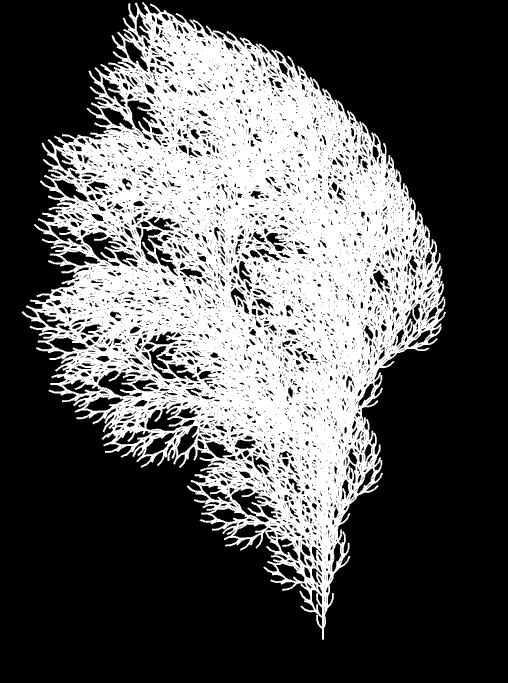
\includegraphics{tree.png}
\caption{tree}
\end{figure}

\begin{Shaded}
\begin{Highlighting}[]
\OtherTok{bush ::} \DataTypeTok{LGrammar}
\NormalTok{bush  }\FunctionTok{=} \NormalTok{(}\DataTypeTok{Lg} \StringTok{"A"}
         \NormalTok{[}\DataTypeTok{Pr} \StringTok{"A"} \StringTok{"[&FL!A]/////'[&FL!A]///////'[&FL!A]"}\NormalTok{,}
          \DataTypeTok{Pr} \StringTok{"F"} \StringTok{"S ///// F"}\NormalTok{,}
          \DataTypeTok{Pr} \StringTok{"S"} \StringTok{"F L"}\NormalTok{,}
          \DataTypeTok{Pr} \StringTok{"L"} \StringTok{"['''^^\{-f+f+f-\textbar{}-f+f+f\}]"}\NormalTok{])}
\end{Highlighting}
\end{Shaded}
\begin{figure}[htbp]
\centering
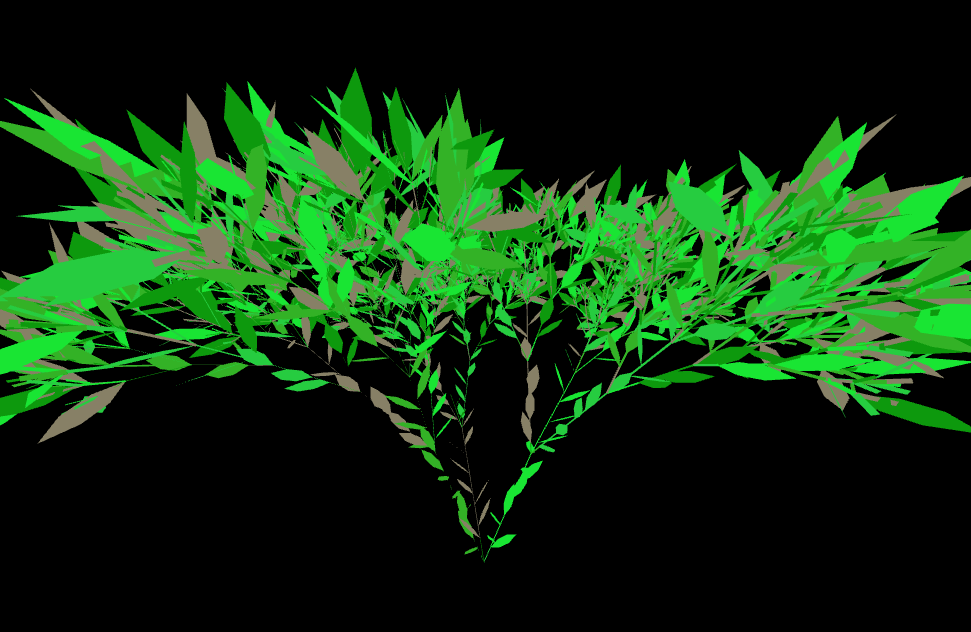
\includegraphics{bush.png}
\caption{bush}
\end{figure}

\begin{Shaded}
\begin{Highlighting}[]
\OtherTok{plant ::} \DataTypeTok{LGrammar}
\NormalTok{plant  }\FunctionTok{=} \NormalTok{(}\DataTypeTok{Lg} \StringTok{"P"}
          \NormalTok{[}\DataTypeTok{Pr} \StringTok{"P"} \StringTok{"i+[P+o]--//[--l]i[++l]-[Po]++PF"}\NormalTok{,}
           \DataTypeTok{Pr} \StringTok{"i"} \StringTok{"Fs[//&&l][//^^l]Fs"}\NormalTok{,}
           \DataTypeTok{Pr} \StringTok{"s"} \StringTok{"FsF"}\NormalTok{,}
           \DataTypeTok{Pr} \StringTok{"l"} \StringTok{"['\{+f-ff-f+\textbar{}+f-ff-f\}]"}\NormalTok{,}
           \DataTypeTok{Pr} \StringTok{"o"} \StringTok{"[&&&c'/w////w////w////w////w]"}\NormalTok{,}
           \DataTypeTok{Pr} \StringTok{"c"} \StringTok{"FF"}\NormalTok{,}
           \DataTypeTok{Pr} \StringTok{"w"} \StringTok{"['^F][\{&&&&-f+f\textbar{}-f+f\}]"}\NormalTok{])}
\end{Highlighting}
\end{Shaded}
\begin{figure}[htbp]
\centering
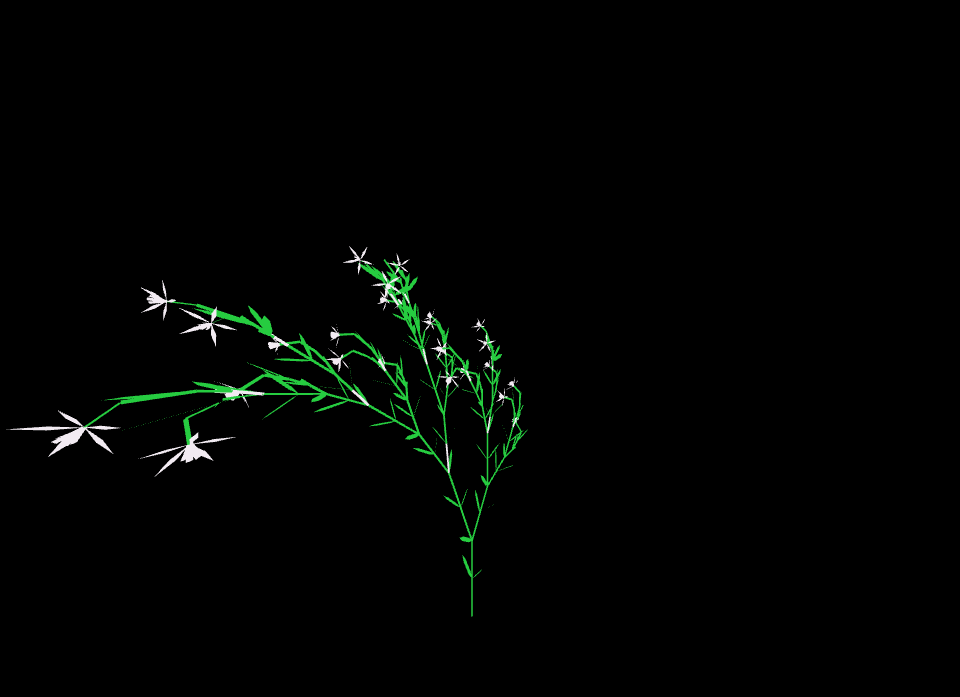
\includegraphics{plant.png}
\caption{plant}
\end{figure}

Now, \texttt{drawScene} is the core loop of the program. It takes a
String of turtle commands and an IORef which represents the current
angle of rotation at which to display the LSystem. It works by clearing
the OpenGL context, translating and rotating the drawing matrix, and
then \texttt{interpret}ing the string of commands to actually do the
drawing. It then updates the rotation angle and flushes commands to
OpenGL.

\begin{Shaded}
\begin{Highlighting}[]
\OtherTok{drawScene ::} \DataTypeTok{String} \OtherTok{->} \DataTypeTok{IORef} \DataTypeTok{Scalar} \OtherTok{->} \DataTypeTok{IO} \NormalTok{()}
\NormalTok{drawScene s rtheta }\FunctionTok{=} \KeywordTok{do}
  \NormalTok{glClear }\FunctionTok{$} \FunctionTok{fromIntegral}  \FunctionTok{$}  \NormalTok{gl_COLOR_BUFFER_BIT}
                         \FunctionTok{.\textbar{}.} \NormalTok{gl_DEPTH_BUFFER_BIT}
  \NormalTok{glLoadIdentity}
  \NormalTok{th }\OtherTok{<-} \NormalTok{readIORef rtheta}
  \NormalTok{glTranslatef (}\DecValTok{0}\NormalTok{) (}\FunctionTok{-}\DecValTok{100}\NormalTok{) (}\FunctionTok{-}\DecValTok{80}\NormalTok{)}
  \NormalTok{glRotatef th }\DecValTok{0} \DecValTok{1} \DecValTok{0}
  \NormalTok{_ }\OtherTok{<-} \NormalTok{interpret s }\FloatTok{22.5}
  \NormalTok{writeIORef rtheta }\FunctionTok{$!} \NormalTok{th }\FunctionTok{+} \FloatTok{0.5}
  \NormalTok{glFlush}
\end{Highlighting}
\end{Shaded}
\section{Summary}

That, barring some OpenGL glue code, is the main body of work for this
project. In many ways, I found this deeply satisfying, because it is by
far the most complete implementation of L-Systems and turtle graphics I
have ever successfully written. For many years I have wanted to build
this, and I'm proud of what I've achieved.

I would very much like to do more -- especially in the way of expanding
the supported grammars, such as context-sensitive, stochastic, and
parametric productions. Some of these seem within reach (such as
stochasticism) and others seem like they may have to wait a while --
like fully context-sensitive productions.

Creating this software in Haskell has been a very pleasant experience
overall. I enjoy that Haskell has such strong opinions about code and
how it should be structured, because it pushes me toward that ideal and
encourages me to think harder about what I'm writing and how it should
be expressed. I have several lingering refactors and enhancements I'd
like to undertake, such as:

\begin{itemize}
\item
  splitting up the \texttt{generate} function and promoting some of the
  helper functions to the top level
\item
  attempting a combinatoric approach to productions rather than a data-
  driven approach
\item
  using Parsec to add support for an external file format
\item
  adding support for user interaction with the 3d model
\end{itemize}
\subsection{Bibliography}

\emph{The Algorithmic Beauty of Plants}, by Aristid Lindenmayer and
Przemyslaw Pruszinkiewicz.

\subsection{OpenGL Utiltity Functions}

These were borrowed rather wholesale from a
\href{http://hackage.haskell.org/package/nehe-tuts}{Haskell port} of the
very useful \href{http://nehe.gamedev.net/}{Neon-Helium OpenGL
tutorials} of yore (for values of yore in the neighborhood of 1999).

I have modified them slightly from the code in Hackage, though not
substantially.

\begin{Shaded}
\begin{Highlighting}[]
\OtherTok{setupGraphics              ::} \DataTypeTok{Int} \OtherTok{->} \DataTypeTok{Int} \OtherTok{->} \DataTypeTok{IO} \NormalTok{()}
\NormalTok{setupGraphics w h }\FunctionTok{=} \KeywordTok{do}
  \NormalTok{r }\OtherTok{<-} \NormalTok{newIORef }\DecValTok{0}
  \KeywordTok{True} \OtherTok{<-} \NormalTok{GLFW.initialize}
  \CommentTok{-- select type of display mode:}
  \CommentTok{-- Double buffer}
  \CommentTok{-- RGBA color}
  \CommentTok{-- Alpha components supported}
  \CommentTok{-- Depth buffer}
  \KeywordTok{let} \NormalTok{dspOpts }\FunctionTok{=} \NormalTok{GLFW.defaultDisplayOptions}
                \NormalTok{\{ GLFW.displayOptions_width  }\FunctionTok{=} \NormalTok{w}
                \NormalTok{, GLFW.displayOptions_height }\FunctionTok{=} \NormalTok{h}
                \CommentTok{-- Set depth buffering and RGBA colors}
                \NormalTok{, GLFW.displayOptions_numRedBits   }\FunctionTok{=} \DecValTok{8}
                \NormalTok{, GLFW.displayOptions_numGreenBits }\FunctionTok{=} \DecValTok{8}
                \NormalTok{, GLFW.displayOptions_numBlueBits  }\FunctionTok{=} \DecValTok{8}
                \NormalTok{, GLFW.displayOptions_numAlphaBits }\FunctionTok{=} \DecValTok{8}
                \NormalTok{, GLFW.displayOptions_numDepthBits }\FunctionTok{=} \DecValTok{8}
                \NormalTok{, GLFW.displayOptions_numFsaaSamples }\FunctionTok{=} \KeywordTok{Just} \DecValTok{8}
                \CommentTok{-- , GLFW.displayOptions_displayMode = GLFW.Fullscreen}
                \NormalTok{\}}
  \CommentTok{-- open a window}
  \KeywordTok{True} \OtherTok{<-} \NormalTok{GLFW.openWindow dspOpts}
  \CommentTok{-- window starts at upper left corner of the screen}
  \NormalTok{GLFW.setWindowPosition }\DecValTok{0} \DecValTok{0}
  \NormalTok{GLFW.setWindowTitle }\StringTok{"ls-hs"}
  \CommentTok{-- register the function to do all our OpenGL drawing}
  \KeywordTok{let} \NormalTok{s }\FunctionTok{=} \NormalTok{(generate tree }\DecValTok{5}\NormalTok{)}
  \NormalTok{GLFW.setWindowRefreshCallback (drawScene s r)}
  \CommentTok{-- GLFW.setWindowRefreshCallback (drawScene rt rq)}
  \CommentTok{-- register the funciton called when our window is resized}
  \NormalTok{GLFW.setWindowSizeCallback resizeScene}
  \CommentTok{-- register the function called when the keyboard is pressed.}
  \NormalTok{GLFW.setKeyCallback keyPressed}
  \NormalTok{GLFW.setWindowCloseCallback shutdown}
  \CommentTok{-- initialize our window.}
  \NormalTok{initGL}
  \NormalTok{forever }\FunctionTok{$} \KeywordTok{do}
    \NormalTok{drawScene s r}
    \NormalTok{GLFW.swapBuffers}
\end{Highlighting}
\end{Shaded}
\begin{Shaded}
\begin{Highlighting}[]
\OtherTok{initGL ::} \DataTypeTok{IO} \NormalTok{()}
\NormalTok{initGL }\FunctionTok{=} \KeywordTok{do}
  \NormalTok{glShadeModel gl_SMOOTH }\CommentTok{-- enables smooth color shading}
  \NormalTok{glClearColor }\DecValTok{0} \DecValTok{0} \DecValTok{0} \DecValTok{0} \CommentTok{-- Clear the background color to black}
  \NormalTok{glClearDepth }\DecValTok{1} \CommentTok{-- enables clearing of the depth buffer}
  \NormalTok{glEnable gl_DEPTH_TEST}
  \NormalTok{glDepthFunc gl_LEQUAL  }\CommentTok{-- type of depth test}
  \NormalTok{glHint gl_PERSPECTIVE_CORRECTION_HINT gl_NICEST}
\end{Highlighting}
\end{Shaded}
\begin{Shaded}
\begin{Highlighting}[]
\OtherTok{resizeScene ::} \DataTypeTok{GLFW.WindowSizeCallback}
\NormalTok{resizeScene w     }\DecValTok{0}      \FunctionTok{=} \NormalTok{resizeScene w }\DecValTok{1} \CommentTok{-- prevent divide by zero}
\NormalTok{resizeScene w h }\FunctionTok{=} \KeywordTok{do}
  \NormalTok{glViewport }\DecValTok{0} \DecValTok{0} \NormalTok{(}\FunctionTok{fromIntegral} \NormalTok{w) (}\FunctionTok{fromIntegral} \NormalTok{h)}
  \NormalTok{glMatrixMode gl_PROJECTION}
  \NormalTok{glLoadIdentity}
  \NormalTok{gluPerspective }\DecValTok{120} \NormalTok{(}\FunctionTok{fromIntegral} \NormalTok{w }\FunctionTok{/} \FunctionTok{fromIntegral} \NormalTok{h) }\FloatTok{0.01} \DecValTok{200}
  \NormalTok{glMatrixMode gl_MODELVIEW}
  \NormalTok{glLoadIdentity}
  \NormalTok{glFlush}
\end{Highlighting}
\end{Shaded}
\begin{Shaded}
\begin{Highlighting}[]
\OtherTok{shutdown ::} \DataTypeTok{GLFW.WindowCloseCallback}
\NormalTok{shutdown }\FunctionTok{=} \KeywordTok{do}
  \NormalTok{GLFW.closeWindow}
  \NormalTok{GLFW.terminate}
  \NormalTok{_ }\OtherTok{<-} \NormalTok{exitWith }\DataTypeTok{ExitSuccess}
  \FunctionTok{return} \KeywordTok{True}
\end{Highlighting}
\end{Shaded}
\begin{Shaded}
\begin{Highlighting}[]
\OtherTok{keyPressed                  ::} \DataTypeTok{GLFW.KeyCallback}
\NormalTok{keyPressed }\DataTypeTok{GLFW.KeyEsc} \KeywordTok{True}  \FunctionTok{=} \NormalTok{shutdown }\FunctionTok{>>} \FunctionTok{return} \NormalTok{()}
\NormalTok{keyPressed _           _     }\FunctionTok{=} \FunctionTok{return} \NormalTok{()}
\end{Highlighting}
\end{Shaded}
\begin{Shaded}
\begin{Highlighting}[]
\OtherTok{main ::} \DataTypeTok{IO} \NormalTok{()}
\NormalTok{main }\FunctionTok{=} \KeywordTok{do}
  \NormalTok{setupGraphics }\DecValTok{1000} \DecValTok{750}
\end{Highlighting}
\end{Shaded}

\end{document}
